% Options for packages loaded elsewhere
\PassOptionsToPackage{unicode}{hyperref}
\PassOptionsToPackage{hyphens}{url}
%
\documentclass[
]{book}
\usepackage{amsmath,amssymb}
\usepackage{lmodern}
\usepackage{iftex}
\ifPDFTeX
  \usepackage[T1]{fontenc}
  \usepackage[utf8]{inputenc}
  \usepackage{textcomp} % provide euro and other symbols
\else % if luatex or xetex
  \usepackage{unicode-math}
  \defaultfontfeatures{Scale=MatchLowercase}
  \defaultfontfeatures[\rmfamily]{Ligatures=TeX,Scale=1}
\fi
% Use upquote if available, for straight quotes in verbatim environments
\IfFileExists{upquote.sty}{\usepackage{upquote}}{}
\IfFileExists{microtype.sty}{% use microtype if available
  \usepackage[]{microtype}
  \UseMicrotypeSet[protrusion]{basicmath} % disable protrusion for tt fonts
}{}
\makeatletter
\@ifundefined{KOMAClassName}{% if non-KOMA class
  \IfFileExists{parskip.sty}{%
    \usepackage{parskip}
  }{% else
    \setlength{\parindent}{0pt}
    \setlength{\parskip}{6pt plus 2pt minus 1pt}}
}{% if KOMA class
  \KOMAoptions{parskip=half}}
\makeatother
\usepackage{xcolor}
\usepackage{color}
\usepackage{fancyvrb}
\newcommand{\VerbBar}{|}
\newcommand{\VERB}{\Verb[commandchars=\\\{\}]}
\DefineVerbatimEnvironment{Highlighting}{Verbatim}{commandchars=\\\{\}}
% Add ',fontsize=\small' for more characters per line
\usepackage{framed}
\definecolor{shadecolor}{RGB}{248,248,248}
\newenvironment{Shaded}{\begin{snugshade}}{\end{snugshade}}
\newcommand{\AlertTok}[1]{\textcolor[rgb]{0.94,0.16,0.16}{#1}}
\newcommand{\AnnotationTok}[1]{\textcolor[rgb]{0.56,0.35,0.01}{\textbf{\textit{#1}}}}
\newcommand{\AttributeTok}[1]{\textcolor[rgb]{0.77,0.63,0.00}{#1}}
\newcommand{\BaseNTok}[1]{\textcolor[rgb]{0.00,0.00,0.81}{#1}}
\newcommand{\BuiltInTok}[1]{#1}
\newcommand{\CharTok}[1]{\textcolor[rgb]{0.31,0.60,0.02}{#1}}
\newcommand{\CommentTok}[1]{\textcolor[rgb]{0.56,0.35,0.01}{\textit{#1}}}
\newcommand{\CommentVarTok}[1]{\textcolor[rgb]{0.56,0.35,0.01}{\textbf{\textit{#1}}}}
\newcommand{\ConstantTok}[1]{\textcolor[rgb]{0.00,0.00,0.00}{#1}}
\newcommand{\ControlFlowTok}[1]{\textcolor[rgb]{0.13,0.29,0.53}{\textbf{#1}}}
\newcommand{\DataTypeTok}[1]{\textcolor[rgb]{0.13,0.29,0.53}{#1}}
\newcommand{\DecValTok}[1]{\textcolor[rgb]{0.00,0.00,0.81}{#1}}
\newcommand{\DocumentationTok}[1]{\textcolor[rgb]{0.56,0.35,0.01}{\textbf{\textit{#1}}}}
\newcommand{\ErrorTok}[1]{\textcolor[rgb]{0.64,0.00,0.00}{\textbf{#1}}}
\newcommand{\ExtensionTok}[1]{#1}
\newcommand{\FloatTok}[1]{\textcolor[rgb]{0.00,0.00,0.81}{#1}}
\newcommand{\FunctionTok}[1]{\textcolor[rgb]{0.00,0.00,0.00}{#1}}
\newcommand{\ImportTok}[1]{#1}
\newcommand{\InformationTok}[1]{\textcolor[rgb]{0.56,0.35,0.01}{\textbf{\textit{#1}}}}
\newcommand{\KeywordTok}[1]{\textcolor[rgb]{0.13,0.29,0.53}{\textbf{#1}}}
\newcommand{\NormalTok}[1]{#1}
\newcommand{\OperatorTok}[1]{\textcolor[rgb]{0.81,0.36,0.00}{\textbf{#1}}}
\newcommand{\OtherTok}[1]{\textcolor[rgb]{0.56,0.35,0.01}{#1}}
\newcommand{\PreprocessorTok}[1]{\textcolor[rgb]{0.56,0.35,0.01}{\textit{#1}}}
\newcommand{\RegionMarkerTok}[1]{#1}
\newcommand{\SpecialCharTok}[1]{\textcolor[rgb]{0.00,0.00,0.00}{#1}}
\newcommand{\SpecialStringTok}[1]{\textcolor[rgb]{0.31,0.60,0.02}{#1}}
\newcommand{\StringTok}[1]{\textcolor[rgb]{0.31,0.60,0.02}{#1}}
\newcommand{\VariableTok}[1]{\textcolor[rgb]{0.00,0.00,0.00}{#1}}
\newcommand{\VerbatimStringTok}[1]{\textcolor[rgb]{0.31,0.60,0.02}{#1}}
\newcommand{\WarningTok}[1]{\textcolor[rgb]{0.56,0.35,0.01}{\textbf{\textit{#1}}}}
\usepackage{longtable,booktabs,array}
\usepackage{calc} % for calculating minipage widths
% Correct order of tables after \paragraph or \subparagraph
\usepackage{etoolbox}
\makeatletter
\patchcmd\longtable{\par}{\if@noskipsec\mbox{}\fi\par}{}{}
\makeatother
% Allow footnotes in longtable head/foot
\IfFileExists{footnotehyper.sty}{\usepackage{footnotehyper}}{\usepackage{footnote}}
\makesavenoteenv{longtable}
\usepackage{graphicx}
\makeatletter
\def\maxwidth{\ifdim\Gin@nat@width>\linewidth\linewidth\else\Gin@nat@width\fi}
\def\maxheight{\ifdim\Gin@nat@height>\textheight\textheight\else\Gin@nat@height\fi}
\makeatother
% Scale images if necessary, so that they will not overflow the page
% margins by default, and it is still possible to overwrite the defaults
% using explicit options in \includegraphics[width, height, ...]{}
\setkeys{Gin}{width=\maxwidth,height=\maxheight,keepaspectratio}
% Set default figure placement to htbp
\makeatletter
\def\fps@figure{htbp}
\makeatother
\setlength{\emergencystretch}{3em} % prevent overfull lines
\providecommand{\tightlist}{%
  \setlength{\itemsep}{0pt}\setlength{\parskip}{0pt}}
\setcounter{secnumdepth}{5}
\usepackage{booktabs}
\ifLuaTeX
  \usepackage{selnolig}  % disable illegal ligatures
\fi
\usepackage[]{natbib}
\bibliographystyle{apalike}
\IfFileExists{bookmark.sty}{\usepackage{bookmark}}{\usepackage{hyperref}}
\IfFileExists{xurl.sty}{\usepackage{xurl}}{} % add URL line breaks if available
\urlstyle{same} % disable monospaced font for URLs
\hypersetup{
  pdftitle={Technical Manual on Soil Sampling Design.},
  pdfauthor={Rodríguez Lado, L., Angelini, M.E, Naypewe, N., Luotto, I., Yigini, Y.},
  hidelinks,
  pdfcreator={LaTeX via pandoc}}

\title{Technical Manual on Soil Sampling Design.}
\author{\emph{Rodríguez Lado, L., Angelini, M.E, Naypewe, N., Luotto, I., Yigini, Y.}}
\date{2023-12-03}

\begin{document}
\maketitle

{
\setcounter{tocdepth}{1}
\tableofcontents
}
\hypertarget{licence}{%
\chapter*{Licence}\label{licence}}
\addcontentsline{toc}{chapter}{Licence}

The NLSDR Guideline Manual is made available under the Creative Commons Attribution-NonCommercial-ShareAlike 3.0 IGO licence

\href{https://creativecommons.org/licenses/by-nc-sa/3.0/igo/legalcode}{CC BY-NC-SA 3.0 IGO}.

\hypertarget{introduction}{%
\chapter{Introduction}\label{introduction}}

Data can be found at the \href{https://bitbucket.org/brendo1001/clhc_sampling/src/master/}{repository}. A sample script is located at \url{https://bitbucket.org/brendo1001/clhc_sampling/}

\hypertarget{conditioned-latin-hypercube-sampling-clhs}{%
\section*{Conditioned Latin Hypercube Sampling (cLHS)}\label{conditioned-latin-hypercube-sampling-clhs}}
\addcontentsline{toc}{section}{Conditioned Latin Hypercube Sampling (cLHS)}

Conditioned Latin Hypercube Sampling (cLHS) is an advanced statistical method used for sampling multidimensional data developed within the context of digital Soil Mapping. It's an extension of the basic Latin Hypercube Sampling (LHS) technique, a statistical method for generating a distribution of samples of a random variable. The main advantage of LHS over simple random sampling is its ability to ensure that the entire range of the auxiliary variables are explored. It divides the range of each variable into intervals of equal probability and samples each interval.

The term ``conditioned'' refers to the way the sampling is adapted or conditioned based on specific requirements or constraints. It often involves conditioning the sampling process on one or more additional variables or criteria. This helps in generating samples that are not just representative in terms of the range of values, but also in terms of their relationships or distributions. cLHS is particularly useful for sampling from multivariate data, where there are multiple interrelated variables as it occurs in soil surveys. The main advantage of cLHS is its efficiency in sampling and its ability to better capture the structure and relationships within the data, compared to simpler sampling methods, and ensures that the samples are representative not just of the range of each variable, but also of their interrelations. Detailed information on cLHS can be found in \citep{minasny2006}

cHLS is also used to determine the optimal number of samples that cover the entire auxiliary data variability.

\hypertarget{part-part-one---soil-legacy-data}{%
\part*{Part one - Soil Legacy Data}\label{part-part-one---soil-legacy-data}}
\addcontentsline{toc}{part}{Part one - Soil Legacy Data}

\hypertarget{legacy_data}{%
\chapter{Evaluating Soil Legacy Data Sampling for DSM}\label{legacy_data}}

Modelling techniques in Digital Soil Mapping involve the use of sampling point soil data, with its associated soil properties database, and a number of environmental covariates that will be used to ascertain the relationships of soil properties and the environment to then generalize the findings to locations where no samples have been compiled.

In soil sampling design, a crucial issue is to determine both the locations and the number of the samples to be compiled. In an optimal situation, soil sample database should adequately cover all the environmental diversity space in the study area with a frequency relative to the extent of the diversity in the environmental covariates.

When dealing with legacy soil data, a question that arises is if the data is representative of the environmental diversity within the study area. In this Chapter we present a method to answer this question and to build an alternative how many samples can be retrieved to cover the same environmental space as the existing soil data. The method follows the main findings in \citep{Malone} and developed as \texttt{R} scripts.

We adapted the original scripts to make use of vector \texttt{shp} and raster \texttt{tif} files, as these are data formats commonly used by GIS analysts and in which both soil and environmental data is often stored. We also made some changes in order to simplify the number of R packages and to avoid the use of deprecated packages as it appears in the original code.

\hypertarget{data-preparation}{%
\section{Data Preparation}\label{data-preparation}}

We must first load the required packages and data for the analyses. We make use of the packages \texttt{sp} and \texttt{terra} to manipulate spatial data, \texttt{clhs} for Conditioned Latin Hypercube Sampling, \texttt{entropy} to compute Kullback-Leibler (KL) divergence indexes, \texttt{tripack} for Delaunay triangulation and \texttt{manipulate} for interactive plotting within RStudio. Ensure that all these packages are installed in your system before the execution of the script.

In this manual we recommend to use a common structure for the project, where R scripts appear in the root of the working directory and data files are in a \texttt{data/} directory within the root directory (\texttt{shp} and \texttt{tif} files should be within the sub folders \texttt{data/shapes} and \texttt{data/rasters} respectively. Following this recommendation simplifies the definition of paths and execution of the scripts. If users want to change their storage paths they have to be properly adjusted in the script.

We define the working directory to the directory in which the actual file is located and load the soil legacy sampling points and the environmental rasters from the \texttt{data} folder. To avoid the definition of each environmental covariate, we first retrieve all files with the \texttt{.tif} extension and then create a \texttt{SpatRaster} object with all of them in a row.

\begin{Shaded}
\begin{Highlighting}[]
\CommentTok{\# Set working directory to source file location}
  \FunctionTok{setwd}\NormalTok{(}\FunctionTok{dirname}\NormalTok{(rstudioapi}\SpecialCharTok{::}\FunctionTok{getActiveDocumentContext}\NormalTok{()}\SpecialCharTok{$}\NormalTok{path))}
\end{Highlighting}
\end{Shaded}

\begin{Shaded}
\begin{Highlighting}[]
\DocumentationTok{\#\# Load soil legacy point data}
\NormalTok{  p.dat }\OtherTok{\textless{}{-}}\NormalTok{ terra}\SpecialCharTok{::}\FunctionTok{vect}\NormalTok{(}\StringTok{"data/shapes/legacy\_soils.shp"}\NormalTok{)}

\DocumentationTok{\#\# Load raster covariate data{-}{-}{-}{-}}
  \CommentTok{\# Read Spatial data covariates as rasters with terra}
\NormalTok{  rasters }\OtherTok{\textless{}{-}} \StringTok{"data/rasters"}
\NormalTok{  cov.dat }\OtherTok{\textless{}{-}}  \FunctionTok{list.files}\NormalTok{(rasters, }\AttributeTok{pattern =} \StringTok{"tif$"}\NormalTok{,  }\AttributeTok{recursive =} \ConstantTok{TRUE}\NormalTok{, }\AttributeTok{full.names =} \ConstantTok{TRUE}\NormalTok{)}
\NormalTok{  cov.dat }\OtherTok{\textless{}{-}}\NormalTok{ terra}\SpecialCharTok{::}\FunctionTok{rast}\NormalTok{(cov.dat)}
\end{Highlighting}
\end{Shaded}

\begin{Shaded}
\begin{Highlighting}[]
   \FunctionTok{plot}\NormalTok{(cov.dat)}
\end{Highlighting}
\end{Shaded}

\begin{figure}
\centering
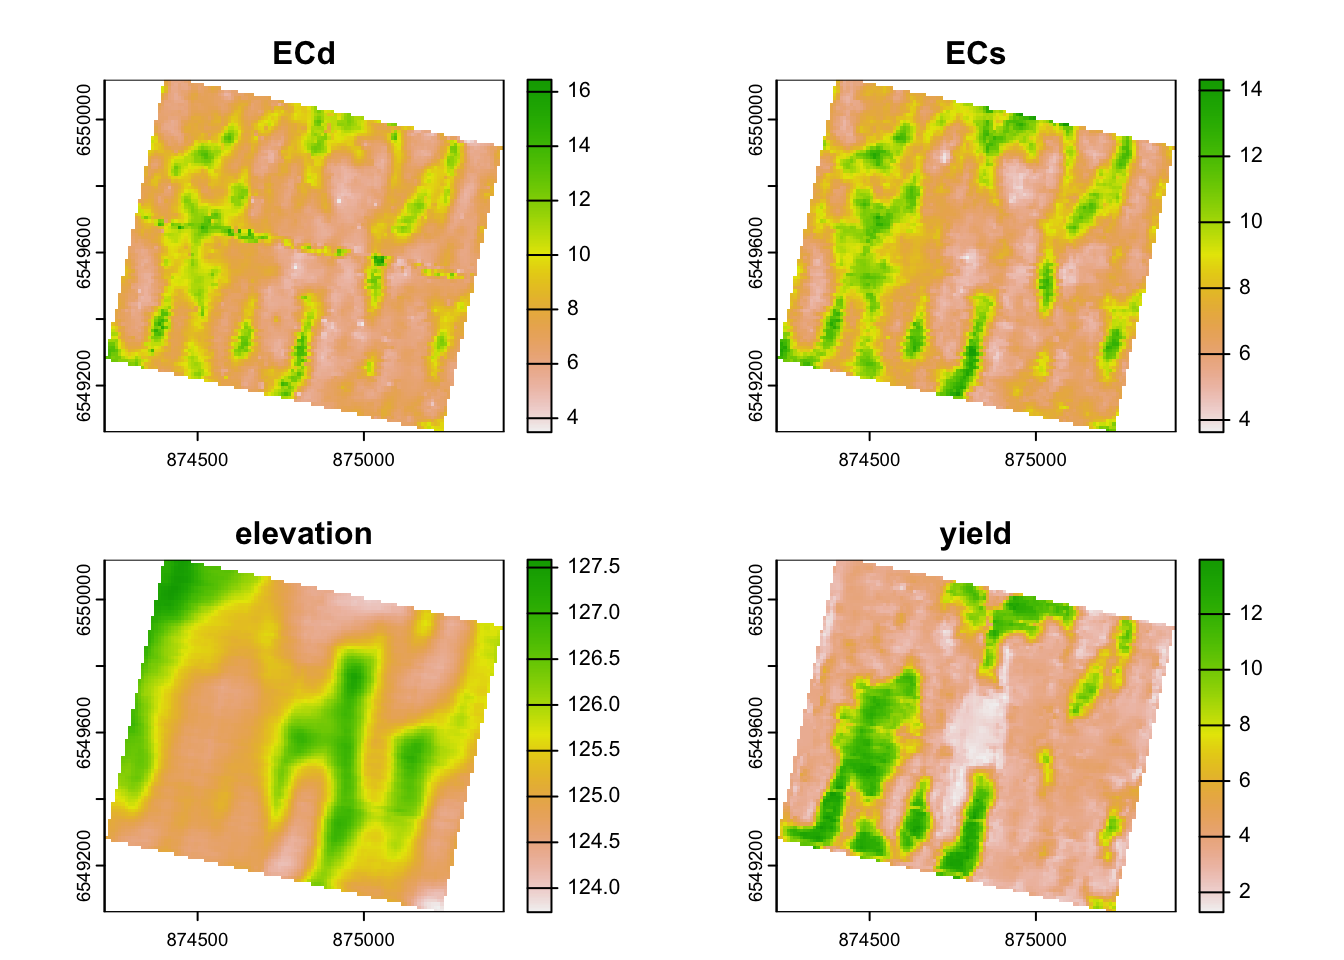
\includegraphics{Technical_Manual-on-Sampling-Design_files/figure-latex/plot_covdata-1.pdf}
\caption{(\#fig:plot\_covdata)Plot of the covariates}
\end{figure}

\hypertarget{representativeness-of-the-legacy-soil-data}{%
\section{Representativeness of the Legacy Soil Data}\label{representativeness-of-the-legacy-soil-data}}

The next step involves the determination of the distributions of environmental values in the soil samples data and its comparison with the existing distributions of each environmental variable to determine the representativeness of the soil points in the environmental space.

The comparison of distributions is performed through the Kullback-Leibler divergence (KL). It is a measure used to quantify the difference between two probability distributions.
KL-divergence compares an ``objective'' or reference probability distribution (here, the distribution of covariates in the complete covariate space - P) with a ``model'' or approximate probability distribution (the space of covariates in the soil samples - Q). The main idea is to determine how much information is lost when Q is used to approximate P. In other words, KL-divergence measures how much the Q distribution deviates from the P distribution.

We cross soil and environmental data to create a dataset with the values of the environmental parameters at the locations of the soil samples.

\begin{Shaded}
\begin{Highlighting}[]
\CommentTok{\# Extract environmental data from rasters at soil locations {-}{-}{-}{-}}
\NormalTok{  p.dat\_I }\OtherTok{\textless{}{-}}\NormalTok{ terra}\SpecialCharTok{::}\FunctionTok{extract}\NormalTok{(cov.dat, p.dat)}
\NormalTok{  p.dat\_I }\OtherTok{\textless{}{-}} \FunctionTok{na.omit}\NormalTok{(p.dat\_I) }\CommentTok{\# Remove soil points outside study area}
  \FunctionTok{str}\NormalTok{(p.dat\_I)}
\end{Highlighting}
\end{Shaded}

\begin{verbatim}
## 'data.frame':    238 obs. of  5 variables:
##  $ ID       : num  1 2 3 4 5 6 7 8 9 10 ...
##  $ ECd      : num  7.48 5.86 7.4 6.84 6.2 ...
##  $ ECs      : num  7.86 5.67 7.81 6.99 5.51 ...
##  $ elevation: num  127 127 127 127 127 ...
##  $ yield    : num  3.03 3.79 3.37 2.62 3.69 ...
\end{verbatim}

We first calculate a \texttt{n-matrix} with the values of the covariates dividing their distributions into \texttt{n} equally-spaced bins. Each bin captures the environmental variability within its interval in the total distribution. In this exercise, \texttt{n} equals to 25. The result is a 26×4 matrix, where the rows represent the upper and lower limit of the bin and (thus, 26 rows are required to represent 25 bins), and 4 correspond to the number of variables used as environmental proxies.

\begin{Shaded}
\begin{Highlighting}[]
\CommentTok{\# Define Number of bins}
\NormalTok{  nb}\OtherTok{\textless{}{-}} \DecValTok{25}
  \CommentTok{\#quantile matrix (of the covariate data)}
\NormalTok{  q.mat}\OtherTok{\textless{}{-}} \FunctionTok{matrix}\NormalTok{(}\ConstantTok{NA}\NormalTok{, }\AttributeTok{nrow=}\NormalTok{(nb}\SpecialCharTok{+}\DecValTok{1}\NormalTok{), }\AttributeTok{ncol=} \FunctionTok{nlyr}\NormalTok{(cov.dat))}
\NormalTok{  j}\OtherTok{=}\DecValTok{1}
  \ControlFlowTok{for}\NormalTok{ (i }\ControlFlowTok{in} \DecValTok{1}\SpecialCharTok{:}\FunctionTok{nlyr}\NormalTok{(cov.dat))\{ }\CommentTok{\#note the index start here}
  \CommentTok{\#get a quantile matrix together of the covariates}
\NormalTok{    ran1 }\OtherTok{\textless{}{-}} \FunctionTok{minmax}\NormalTok{(cov.dat[[i]])[}\DecValTok{2}\NormalTok{] }\SpecialCharTok{{-}} \FunctionTok{minmax}\NormalTok{(cov.dat[[i]])[}\DecValTok{1}\NormalTok{]}
\NormalTok{    step1}\OtherTok{\textless{}{-}}\NormalTok{ ran1}\SpecialCharTok{/}\NormalTok{nb }
\NormalTok{    q.mat[,j]}\OtherTok{\textless{}{-}} \FunctionTok{seq}\NormalTok{(}\FunctionTok{minmax}\NormalTok{(cov.dat[[i]])[}\DecValTok{1}\NormalTok{], }\AttributeTok{to =} \FunctionTok{minmax}\NormalTok{(cov.dat[[i]])[}\DecValTok{2}\NormalTok{], }\AttributeTok{by =}\NormalTok{step1)}
\NormalTok{    j}\OtherTok{\textless{}{-}}\NormalTok{ j}\SpecialCharTok{+}\DecValTok{1}\NormalTok{\}}
\end{Highlighting}
\end{Shaded}

From this matrix, we compute the hypercube matrix of covariates in the whole covariate space.

\begin{Shaded}
\begin{Highlighting}[]
\CommentTok{\# Hypercube of "objective" distribution (P) {-} covariates}
\NormalTok{  cov.dat.df }\OtherTok{\textless{}{-}} \FunctionTok{as.data.frame}\NormalTok{(cov.dat) }\CommentTok{\# convert SpatRaster to dataframe}
\NormalTok{  cov.mat}\OtherTok{\textless{}{-}} \FunctionTok{matrix}\NormalTok{(}\DecValTok{1}\NormalTok{, }\AttributeTok{nrow=}\NormalTok{nb, }\AttributeTok{ncol=}\FunctionTok{ncol}\NormalTok{(q.mat))}
    \ControlFlowTok{for}\NormalTok{ (i }\ControlFlowTok{in} \DecValTok{1}\SpecialCharTok{:}\FunctionTok{nrow}\NormalTok{(cov.dat.df))\{ }\CommentTok{\# the number of pixels}
\NormalTok{      cntj}\OtherTok{\textless{}{-}} \DecValTok{1} 
    \ControlFlowTok{for}\NormalTok{ (j }\ControlFlowTok{in} \DecValTok{1}\SpecialCharTok{:}\FunctionTok{ncol}\NormalTok{(cov.dat.df))\{ }\CommentTok{\#for each column}
\NormalTok{      dd}\OtherTok{\textless{}{-}}\NormalTok{ cov.dat.df[i,j]  }
      \ControlFlowTok{for}\NormalTok{ (k }\ControlFlowTok{in} \DecValTok{1}\SpecialCharTok{:}\NormalTok{nb)\{  }\CommentTok{\#for each quantile}
\NormalTok{        kl}\OtherTok{\textless{}{-}}\NormalTok{ q.mat[k, cntj] }
\NormalTok{        ku}\OtherTok{\textless{}{-}}\NormalTok{ q.mat[k}\SpecialCharTok{+}\DecValTok{1}\NormalTok{, cntj] }
        \ControlFlowTok{if}\NormalTok{ (}\FunctionTok{is.na}\NormalTok{(dd)) \{}
          \FunctionTok{print}\NormalTok{(}\StringTok{\textquotesingle{}Missing\textquotesingle{}}\NormalTok{)}
\NormalTok{        \}}
        \ControlFlowTok{else} \ControlFlowTok{if}\NormalTok{ (dd }\SpecialCharTok{\textgreater{}=}\NormalTok{ kl }\SpecialCharTok{\&}\NormalTok{ dd }\SpecialCharTok{\textless{}=}\NormalTok{ ku)\{cov.mat[k, cntj]}\OtherTok{\textless{}{-}}\NormalTok{ cov.mat[k, cntj] }\SpecialCharTok{+} \DecValTok{1}\NormalTok{\} }
\NormalTok{      \}}
\NormalTok{      cntj}\OtherTok{\textless{}{-}}\NormalTok{ cntj}\SpecialCharTok{+}\DecValTok{1}
\NormalTok{    \}}
\NormalTok{  \}}
\end{Highlighting}
\end{Shaded}

We then calculate the hypercube matrix of covariates in the sample space.

\begin{Shaded}
\begin{Highlighting}[]
\CommentTok{\# Sample data hypercube}
\NormalTok{  h.mat}\OtherTok{\textless{}{-}} \FunctionTok{matrix}\NormalTok{(}\DecValTok{1}\NormalTok{, }\AttributeTok{nrow=}\NormalTok{nb, }\AttributeTok{ncol=}\FunctionTok{ncol}\NormalTok{(q.mat))}
  
  \ControlFlowTok{for}\NormalTok{ (ii }\ControlFlowTok{in} \DecValTok{1}\SpecialCharTok{:}\FunctionTok{nrow}\NormalTok{(p.dat\_I))\{ }\CommentTok{\# the number of observations}
\NormalTok{    cntj}\OtherTok{\textless{}{-}} \DecValTok{1} 
    \ControlFlowTok{for}\NormalTok{ (jj }\ControlFlowTok{in} \DecValTok{2}\SpecialCharTok{:}\FunctionTok{ncol}\NormalTok{(p.dat\_I))\{ }\CommentTok{\#for each column}
\NormalTok{      dd}\OtherTok{\textless{}{-}}\NormalTok{ p.dat\_I[ii,jj]  }
      \ControlFlowTok{for}\NormalTok{ (kk }\ControlFlowTok{in} \DecValTok{1}\SpecialCharTok{:}\NormalTok{nb)\{  }\CommentTok{\#for each bin}
\NormalTok{        kl}\OtherTok{\textless{}{-}}\NormalTok{ q.mat[kk, cntj] }
\NormalTok{        ku}\OtherTok{\textless{}{-}}\NormalTok{ q.mat[kk}\SpecialCharTok{+}\DecValTok{1}\NormalTok{, cntj] }
        \ControlFlowTok{if}\NormalTok{ (dd }\SpecialCharTok{\textgreater{}=}\NormalTok{ kl }\SpecialCharTok{\&}\NormalTok{ dd }\SpecialCharTok{\textless{}=}\NormalTok{ ku)\{h.mat[kk, cntj]}\OtherTok{\textless{}{-}}\NormalTok{ h.mat[kk, cntj] }\SpecialCharTok{+} \DecValTok{1}\NormalTok{\}}
\NormalTok{      \}}
\NormalTok{      cntj}\OtherTok{\textless{}{-}}\NormalTok{ cntj}\SpecialCharTok{+}\DecValTok{1}
\NormalTok{    \}}
\NormalTok{  \}}
\end{Highlighting}
\end{Shaded}

\begin{itemize}
\tightlist
\item
  \textbf{KL-divergence}
\end{itemize}

We calculate the KL-divergence to measure how much the distribution of covariates in tbe sample space (Q) deviates from the distribution of covariates in the complete study area space (P).

\begin{Shaded}
\begin{Highlighting}[]
\DocumentationTok{\#\# Compare covariate distributions in P and Q with Kullback{-}Leibler (KL) divergence}
\NormalTok{    kl.index }\OtherTok{\textless{}{-}}\FunctionTok{c}\NormalTok{()}
    \ControlFlowTok{for}\NormalTok{(i }\ControlFlowTok{in} \DecValTok{1}\SpecialCharTok{:}\FunctionTok{ncol}\NormalTok{(cov.dat.df))\{}
\NormalTok{      kl }\OtherTok{\textless{}{-}}    \FunctionTok{KL.empirical}\NormalTok{(}\FunctionTok{c}\NormalTok{(cov.mat[,i]), }\FunctionTok{c}\NormalTok{(h.mat[,i]))}
\NormalTok{      kl.index }\OtherTok{\textless{}{-}} \FunctionTok{c}\NormalTok{(kl.index,kl)}
\NormalTok{      klo }\OtherTok{\textless{}{-}}  \FunctionTok{mean}\NormalTok{(kl.index)}
\NormalTok{    \}}
    \FunctionTok{print}\NormalTok{(kl.index) }\CommentTok{\# KL divergences of each covariate}
\end{Highlighting}
\end{Shaded}

\begin{verbatim}
## [1] 0.04115895 0.04241792 0.02779852 0.04328375
\end{verbatim}

\begin{Shaded}
\begin{Highlighting}[]
    \FunctionTok{print}\NormalTok{(klo) }\CommentTok{\# KL divergence in the existing soil samples}
\end{Highlighting}
\end{Shaded}

\begin{verbatim}
## [1] 0.03866478
\end{verbatim}

The KL-divergence is always greater than or equal to zero, and reaches its minimum value (zero) only when P and Q are identical. Thus, lower values of KL-divergence are indicative of a good match between both the sample and the study area spaces, indicating that the sample space is a fair representation of the environmental conditions in the study area.

In this case, the KL-divergence value is 0.039, indicating that the legacy samples capture most of the environmental variability in the study area.

\begin{itemize}
\tightlist
\item
  \textbf{Percent of representativeness in relation to the overall environmental conditions}
\end{itemize}

Finally, we can also determine the degree in which our legacy soil dataset is representative of the existing environmental conditions in the study area. For that, we calculate the proportion of pixels in the study area that would fall within the convex hull polygon delineated upon the environmental conditions found at the soil legacy data locations only. The convex hull polygon is created upon a Principal Component transformation of the covariate data in the soil legacy data and using the outter limits of the scores of the points projected on the two main Components.

\begin{Shaded}
\begin{Highlighting}[]
\DocumentationTok{\#\#\#\# Representativeness of the Legacy Dataset: {-}{-}{-}{-}}
  \DocumentationTok{\#\# Calculate the proportion of "env. variables" in the covariate spectra that fall within the convex hull of variables in the "environmental sample space"}
  
  \CommentTok{\# Principal component of the legacy data sample}
\NormalTok{    pca.s }\OtherTok{=} \FunctionTok{prcomp}\NormalTok{(p.dat\_I[,}\DecValTok{2}\SpecialCharTok{:}\NormalTok{(}\FunctionTok{ncol}\NormalTok{(cov.dat.df)}\SpecialCharTok{+}\DecValTok{1}\NormalTok{)],}\AttributeTok{scale=}\ConstantTok{TRUE}\NormalTok{, }\AttributeTok{center=}\ConstantTok{TRUE}\NormalTok{)}
\NormalTok{    scores\_pca1 }\OtherTok{=} \FunctionTok{as.data.frame}\NormalTok{(pca.s}\SpecialCharTok{$}\NormalTok{x)}
  \CommentTok{\# Plot the first 2 principal components and convex hull}
\NormalTok{    rand.tr }\OtherTok{\textless{}{-}} \FunctionTok{tri.mesh}\NormalTok{(scores\_pca1[,}\DecValTok{1}\NormalTok{],scores\_pca1[,}\DecValTok{2}\NormalTok{],}\StringTok{"remove"}\NormalTok{) }\CommentTok{\# Delaunay triangulation }
\NormalTok{    rand.ch}\OtherTok{\textless{}{-}}\FunctionTok{convex.hull}\NormalTok{(rand.tr, }\AttributeTok{plot.it=}\NormalTok{F) }\CommentTok{\# convex hull}
\NormalTok{    pr\_poly }\OtherTok{=} \FunctionTok{cbind}\NormalTok{(}\AttributeTok{x=}\FunctionTok{c}\NormalTok{(rand.ch}\SpecialCharTok{$}\NormalTok{x),}\AttributeTok{y=}\FunctionTok{c}\NormalTok{(rand.ch}\SpecialCharTok{$}\NormalTok{y)) }\CommentTok{\# save the convex hull vertices}
    \FunctionTok{plot}\NormalTok{(scores\_pca1[,}\DecValTok{1}\NormalTok{], scores\_pca1[,}\DecValTok{2}\NormalTok{], }\AttributeTok{xlab=}\StringTok{"PCA 1"}\NormalTok{, }\AttributeTok{ylab=}\StringTok{"PCA 2"}\NormalTok{, }\AttributeTok{xlim=}\FunctionTok{c}\NormalTok{(}\FunctionTok{min}\NormalTok{(scores\_pca1[,}\DecValTok{1}\SpecialCharTok{:}\DecValTok{2}\NormalTok{]), }\FunctionTok{max}\NormalTok{(scores\_pca1[,}\DecValTok{1}\SpecialCharTok{:}\DecValTok{2}\NormalTok{])),}\AttributeTok{ylim=}\FunctionTok{c}\NormalTok{(}\FunctionTok{min}\NormalTok{(scores\_pca1[,}\DecValTok{1}\SpecialCharTok{:}\DecValTok{2}\NormalTok{]), }\FunctionTok{max}\NormalTok{(scores\_pca1[,}\DecValTok{1}\SpecialCharTok{:}\DecValTok{2}\NormalTok{])), }\AttributeTok{main=}\StringTok{\textquotesingle{}Convex hull of soil legacy data\textquotesingle{}}\NormalTok{)}
    \FunctionTok{lines}\NormalTok{(}\FunctionTok{c}\NormalTok{(rand.ch}\SpecialCharTok{$}\NormalTok{x,rand.ch}\SpecialCharTok{$}\NormalTok{x[}\DecValTok{1}\NormalTok{]), }\FunctionTok{c}\NormalTok{(rand.ch}\SpecialCharTok{$}\NormalTok{y,rand.ch}\SpecialCharTok{$}\NormalTok{y[}\DecValTok{1}\NormalTok{]),}\AttributeTok{col=}\StringTok{"red"}\NormalTok{,}\AttributeTok{lwd=}\DecValTok{1}\NormalTok{) }\CommentTok{\# draw the convex hull (domain of legacy data)}
\end{Highlighting}
\end{Shaded}

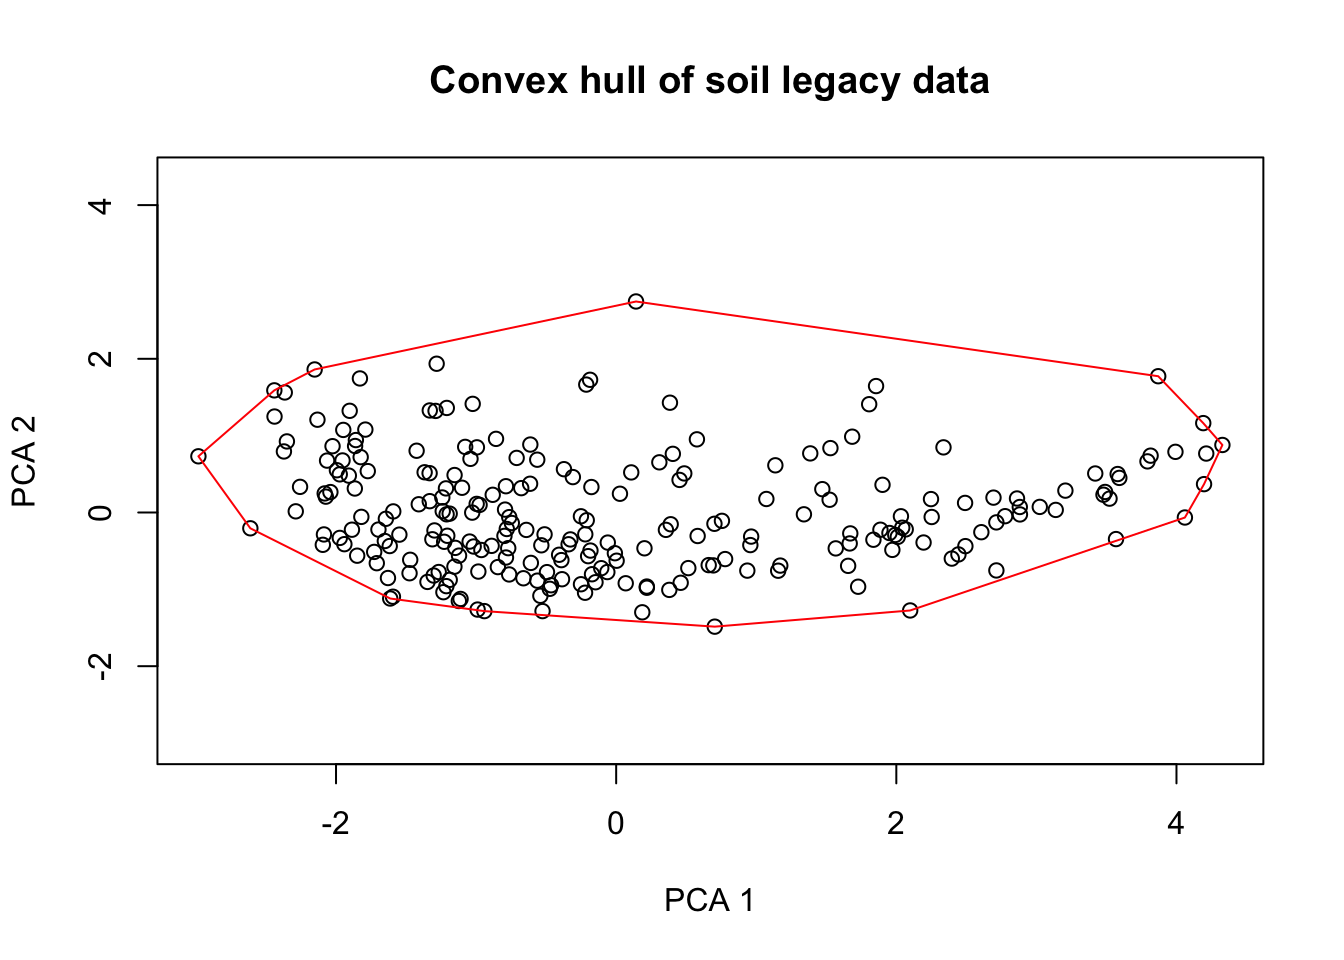
\includegraphics{Technical_Manual-on-Sampling-Design_files/figure-latex/legacy_data_adequacy-1.pdf}

\begin{Shaded}
\begin{Highlighting}[]
  \CommentTok{\# PCA projection of study area population onto the principal components}
\NormalTok{    PCA\_projection}\OtherTok{\textless{}{-}} \FunctionTok{predict}\NormalTok{(pca.s, cov.dat.df) }\CommentTok{\# Project study area population onto sample PC}
\NormalTok{    newScores }\OtherTok{=} \FunctionTok{cbind}\NormalTok{(}\AttributeTok{x=}\NormalTok{PCA\_projection[,}\DecValTok{1}\NormalTok{],}\AttributeTok{y=}\NormalTok{PCA\_projection[,}\DecValTok{2}\NormalTok{]) }\CommentTok{\# PC scores of projected population}
  
  \CommentTok{\# Plot the polygon and all points to be checked}
    \FunctionTok{plot}\NormalTok{(newScores, }\AttributeTok{xlab=}\StringTok{"PCA 1"}\NormalTok{, }\AttributeTok{ylab=}\StringTok{"PCA 2"}\NormalTok{, }\AttributeTok{xlim=}\FunctionTok{c}\NormalTok{(}\FunctionTok{min}\NormalTok{(newScores[,}\DecValTok{1}\SpecialCharTok{:}\DecValTok{2}\NormalTok{]), }\FunctionTok{max}\NormalTok{(newScores[,}\DecValTok{1}\SpecialCharTok{:}\DecValTok{2}\NormalTok{])), }\AttributeTok{ylim=}\FunctionTok{c}\NormalTok{(}\FunctionTok{min}\NormalTok{(newScores[,}\DecValTok{1}\SpecialCharTok{:}\DecValTok{2}\NormalTok{]), }\FunctionTok{max}\NormalTok{(newScores[,}\DecValTok{1}\SpecialCharTok{:}\DecValTok{2}\NormalTok{])), }\AttributeTok{col=}\StringTok{\textquotesingle{}black\textquotesingle{}}\NormalTok{, }\AttributeTok{main=}\StringTok{\textquotesingle{}Environmental space plots over the convex hull of soil legacy data\textquotesingle{}}\NormalTok{)}
    \FunctionTok{polygon}\NormalTok{(pr\_poly,}\AttributeTok{col=}\StringTok{\textquotesingle{}\#99999990\textquotesingle{}}\NormalTok{)}
  \CommentTok{\# Check which points fall within the polygon}
\NormalTok{    pip }\OtherTok{\textless{}{-}} \FunctionTok{point.in.polygon}\NormalTok{(newScores[,}\DecValTok{2}\NormalTok{], newScores[,}\DecValTok{1}\NormalTok{], pr\_poly[,}\DecValTok{2}\NormalTok{],pr\_poly[,}\DecValTok{1}\NormalTok{],}\AttributeTok{mode.checked=}\ConstantTok{FALSE}\NormalTok{)}
\NormalTok{    newScores }\OtherTok{\textless{}{-}} \FunctionTok{data.frame}\NormalTok{(}\FunctionTok{cbind}\NormalTok{(newScores, pip))}
  \CommentTok{\# Plot points outside convex hull  }
    \FunctionTok{points}\NormalTok{(newScores[}\FunctionTok{which}\NormalTok{(newScores}\SpecialCharTok{$}\NormalTok{pip}\SpecialCharTok{==}\DecValTok{0}\NormalTok{),}\DecValTok{1}\SpecialCharTok{:}\DecValTok{2}\NormalTok{],}\AttributeTok{pch=}\StringTok{\textquotesingle{}X\textquotesingle{}}\NormalTok{, }\AttributeTok{col=}\StringTok{\textquotesingle{}red\textquotesingle{}}\NormalTok{)}
\end{Highlighting}
\end{Shaded}

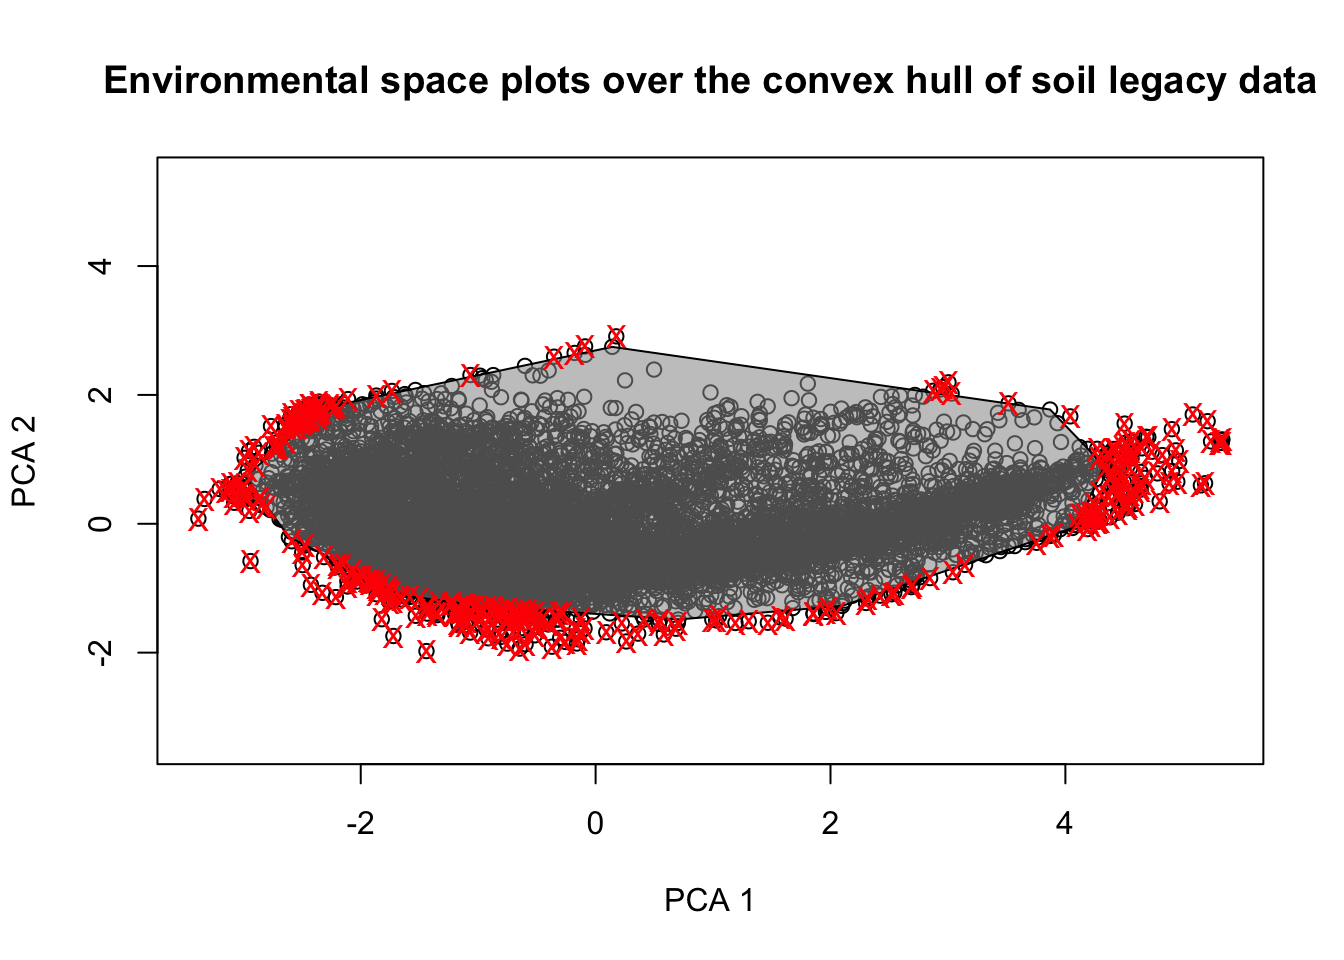
\includegraphics{Technical_Manual-on-Sampling-Design_files/figure-latex/legacy_data_adequacy-2.pdf}

\begin{Shaded}
\begin{Highlighting}[]
  \CommentTok{\# Proportion of the conditions in the study area that fall within the convex hull}
    \FunctionTok{sum}\NormalTok{(newScores}\SpecialCharTok{$}\NormalTok{pip)}\SpecialCharTok{/}\FunctionTok{nrow}\NormalTok{(newScores)}\SpecialCharTok{*}\DecValTok{100} 
\end{Highlighting}
\end{Shaded}

\begin{verbatim}
## [1] 96.50188
\end{verbatim}

This indicates that 96.5\% of the existing conditions in the study area fall within the convex hull delineated with the data in the soil samples, showing the adecquacy of the proposed legacy data for DSM.

\hypertarget{part-part-two---soil-sampling-design}{%
\part{Part two - Soil Sampling Design}\label{part-part-two---soil-sampling-design}}

\hypertarget{creating-a-new-sampling-design}{%
\chapter{Creating a new sampling design}\label{creating-a-new-sampling-design}}

Determining the optimal sample size

We load R packages and define the working directory to the directory in which the actual file is located and load the environmental rasters from the \texttt{data} folder.

\begin{Shaded}
\begin{Highlighting}[]
\CommentTok{\# Load packages as a vector objects}
\NormalTok{  packages }\OtherTok{\textless{}{-}} \FunctionTok{c}\NormalTok{(}\StringTok{"sp"}\NormalTok{, }\StringTok{"terra"}\NormalTok{, }\StringTok{"clhs"}\NormalTok{, }\StringTok{"entropy"}\NormalTok{, }\StringTok{"tripack"}\NormalTok{,}\StringTok{"manipulate"}\NormalTok{,}\StringTok{"dplyr"}\NormalTok{,}\StringTok{"plotly"}\NormalTok{) }\CommentTok{\# Create a vector of packages to use}
  \FunctionTok{lapply}\NormalTok{(packages, require, }\AttributeTok{character.only =} \ConstantTok{TRUE}\NormalTok{) }\CommentTok{\# Load packages}
  \FunctionTok{rm}\NormalTok{(packages) }\CommentTok{\# Remove object to save memory space }

\CommentTok{\# Set working directory to source file location}
  \FunctionTok{setwd}\NormalTok{(}\FunctionTok{dirname}\NormalTok{(rstudioapi}\SpecialCharTok{::}\FunctionTok{getActiveDocumentContext}\NormalTok{()}\SpecialCharTok{$}\NormalTok{path))}
\end{Highlighting}
\end{Shaded}

\begin{Shaded}
\begin{Highlighting}[]
\DocumentationTok{\#\# Load raster covariate data{-}{-}{-}{-}}
  \CommentTok{\# Read Spatial data covariates as rasters with terra}
\NormalTok{  rasters }\OtherTok{\textless{}{-}} \StringTok{"data/rasters"}
\NormalTok{  cov.dat }\OtherTok{\textless{}{-}}  \FunctionTok{list.files}\NormalTok{(rasters, }\AttributeTok{pattern =} \StringTok{"tif$"}\NormalTok{,  }\AttributeTok{recursive =} \ConstantTok{TRUE}\NormalTok{, }\AttributeTok{full.names =} \ConstantTok{TRUE}\NormalTok{)}
\NormalTok{  cov.dat }\OtherTok{\textless{}{-}}\NormalTok{ terra}\SpecialCharTok{::}\FunctionTok{rast}\NormalTok{(cov.dat)}
\end{Highlighting}
\end{Shaded}

\begin{Shaded}
\begin{Highlighting}[]
   \FunctionTok{plot}\NormalTok{(cov.dat)}
\end{Highlighting}
\end{Shaded}

\begin{figure}
\centering
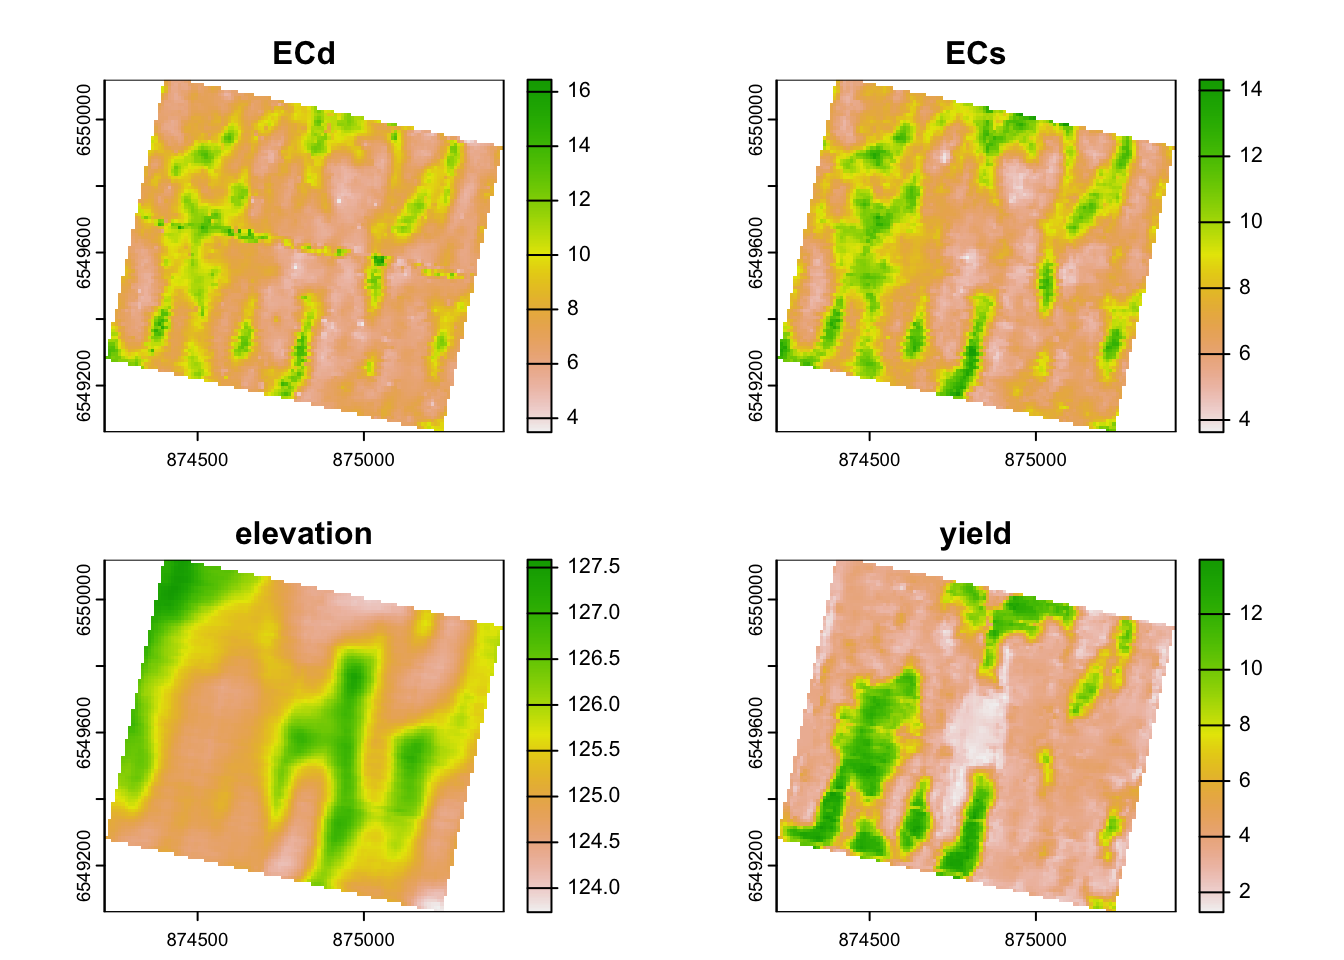
\includegraphics{Technical_Manual-on-Sampling-Design_files/figure-latex/plot_covdata_03-1.pdf}
\caption{(\#fig:plot\_covdata\_03)Plot of the covariates}
\end{figure}

\begin{Shaded}
\begin{Highlighting}[]
  \CommentTok{\# Define empty vectors to store results}
\NormalTok{  number\_of\_samples }\OtherTok{\textless{}{-}} \FunctionTok{c}\NormalTok{()}
\NormalTok{  prop\_explained }\OtherTok{\textless{}{-}} \FunctionTok{c}\NormalTok{()}
\NormalTok{  klo\_samples }\OtherTok{\textless{}{-}}\FunctionTok{c}\NormalTok{()}
    
  \CommentTok{\# Define the number of samples to be tested in a loop (from initial to final) and the step of the sequence}
\NormalTok{  initial.n }\OtherTok{\textless{}{-}} \DecValTok{10}
\NormalTok{  final.n }\OtherTok{\textless{}{-}} \DecValTok{500}
\NormalTok{  by.n }\OtherTok{\textless{}{-}} \DecValTok{20}
\end{Highlighting}
\end{Shaded}

\begin{Shaded}
\begin{Highlighting}[]
  \ControlFlowTok{for}\NormalTok{ (dede }\ControlFlowTok{in} \FunctionTok{seq}\NormalTok{(initial.n, final.n, }\AttributeTok{by=}\NormalTok{by.n))\{}
\NormalTok{    p.dat\_I }\OtherTok{\textless{}{-}} \FunctionTok{spatSample}\NormalTok{(cov.dat,dede, }\AttributeTok{na.rm=}\ConstantTok{TRUE}\NormalTok{,}\AttributeTok{xy=}\ConstantTok{TRUE}\NormalTok{,}\AttributeTok{method=}\StringTok{"random"}\NormalTok{)}
\NormalTok{    p.dat\_I\_sp }\OtherTok{\textless{}{-}}\NormalTok{  p.dat\_I }
    \FunctionTok{coordinates}\NormalTok{(p.dat\_I\_sp)}\OtherTok{\textless{}{-}} \ErrorTok{\textasciitilde{}}\NormalTok{ x }\SpecialCharTok{+}\NormalTok{ y }
\NormalTok{    p.dat\_I }\OtherTok{\textless{}{-}}\NormalTok{ p.dat\_I[}\DecValTok{3}\SpecialCharTok{:}\FunctionTok{ncol}\NormalTok{(p.dat\_I)]}
  
  
  \DocumentationTok{\#\# Comparison of population and sample distributions {-}{-}{-}{-}}
  
    \CommentTok{\# Kullback{-}Leibler (KL) divergence}
    
    \CommentTok{\# Quantiles of the population}
    \CommentTok{\# Number of bins}
\NormalTok{    nb}\OtherTok{\textless{}{-}} \DecValTok{25}
    \CommentTok{\#quantile matrix (of the covariate data)}
\NormalTok{    q.mat}\OtherTok{\textless{}{-}} \FunctionTok{matrix}\NormalTok{(}\ConstantTok{NA}\NormalTok{, }\AttributeTok{nrow=}\NormalTok{(nb}\SpecialCharTok{+}\DecValTok{1}\NormalTok{), }\AttributeTok{ncol=} \FunctionTok{nlyr}\NormalTok{(cov.dat))}
\NormalTok{    j}\OtherTok{=}\DecValTok{1}
    \ControlFlowTok{for}\NormalTok{ (i }\ControlFlowTok{in} \DecValTok{1}\SpecialCharTok{:}\FunctionTok{nlyr}\NormalTok{(cov.dat))\{ }\CommentTok{\#note the index start here}
      \CommentTok{\#get a quantile matrix together of the covariates}
\NormalTok{      ran1 }\OtherTok{\textless{}{-}} \FunctionTok{minmax}\NormalTok{(cov.dat[[i]])[}\DecValTok{2}\NormalTok{] }\SpecialCharTok{{-}} \FunctionTok{minmax}\NormalTok{(cov.dat[[i]])[}\DecValTok{1}\NormalTok{]}
\NormalTok{      step1}\OtherTok{\textless{}{-}}\NormalTok{ ran1}\SpecialCharTok{/}\NormalTok{nb }
\NormalTok{      q.mat[,j]}\OtherTok{\textless{}{-}} \FunctionTok{seq}\NormalTok{(}\FunctionTok{minmax}\NormalTok{(cov.dat[[i]])[}\DecValTok{1}\NormalTok{], }\AttributeTok{to =} \FunctionTok{minmax}\NormalTok{(cov.dat[[i]])[}\DecValTok{2}\NormalTok{], }\AttributeTok{by =}\NormalTok{step1)}
\NormalTok{      j}\OtherTok{\textless{}{-}}\NormalTok{ j}\SpecialCharTok{+}\DecValTok{1}\NormalTok{\}}
\NormalTok{    q.mat}
    
    \CommentTok{\# Hypercube of population}
    
\NormalTok{    cov.dat.df }\OtherTok{\textless{}{-}} \FunctionTok{as.data.frame}\NormalTok{(cov.dat) }\CommentTok{\# convert SpatRaster to dataframe}
\NormalTok{    cov.mat}\OtherTok{\textless{}{-}} \FunctionTok{matrix}\NormalTok{(}\DecValTok{1}\NormalTok{, }\AttributeTok{nrow=}\NormalTok{nb, }\AttributeTok{ncol=}\FunctionTok{ncol}\NormalTok{(q.mat))}
    \ControlFlowTok{for}\NormalTok{ (i }\ControlFlowTok{in} \DecValTok{1}\SpecialCharTok{:}\FunctionTok{nrow}\NormalTok{(cov.dat.df))\{ }\CommentTok{\# the number of pixels}
\NormalTok{      cntj}\OtherTok{\textless{}{-}} \DecValTok{1} 
      \ControlFlowTok{for}\NormalTok{ (j }\ControlFlowTok{in} \DecValTok{1}\SpecialCharTok{:}\FunctionTok{ncol}\NormalTok{(cov.dat.df))\{ }\CommentTok{\#for each column}
\NormalTok{        dd}\OtherTok{\textless{}{-}}\NormalTok{ cov.dat.df[i,j]  }
        \ControlFlowTok{for}\NormalTok{ (k }\ControlFlowTok{in} \DecValTok{1}\SpecialCharTok{:}\NormalTok{nb)\{  }\CommentTok{\#for each quantile}
\NormalTok{          kl}\OtherTok{\textless{}{-}}\NormalTok{ q.mat[k, cntj] }
\NormalTok{          ku}\OtherTok{\textless{}{-}}\NormalTok{ q.mat[k}\SpecialCharTok{+}\DecValTok{1}\NormalTok{, cntj] }
          \ControlFlowTok{if}\NormalTok{ (}\FunctionTok{is.na}\NormalTok{(dd)) \{}
            \FunctionTok{print}\NormalTok{(}\StringTok{\textquotesingle{}Missing\textquotesingle{}}\NormalTok{)}
\NormalTok{          \}}
          \ControlFlowTok{else} \ControlFlowTok{if}\NormalTok{ (dd }\SpecialCharTok{\textgreater{}=}\NormalTok{ kl }\SpecialCharTok{\&}\NormalTok{ dd }\SpecialCharTok{\textless{}=}\NormalTok{ ku)\{cov.mat[k, cntj]}\OtherTok{\textless{}{-}}\NormalTok{ cov.mat[k, cntj] }\SpecialCharTok{+} \DecValTok{1}\NormalTok{\} }
\NormalTok{        \}}
\NormalTok{        cntj}\OtherTok{\textless{}{-}}\NormalTok{ cntj}\SpecialCharTok{+}\DecValTok{1}
\NormalTok{      \}}
\NormalTok{    \}}
\NormalTok{    cov.mat}
    
    
    \CommentTok{\# Compare whole study area covariate space with the selected sample}
    \CommentTok{\# Sample data hypercube (essentially the same script as for the grid data but just doing it on the sample data)}
\NormalTok{    h.mat}\OtherTok{\textless{}{-}} \FunctionTok{matrix}\NormalTok{(}\DecValTok{1}\NormalTok{, }\AttributeTok{nrow=}\NormalTok{nb, }\AttributeTok{ncol=}\FunctionTok{ncol}\NormalTok{(q.mat))}
    
    \ControlFlowTok{for}\NormalTok{ (ii }\ControlFlowTok{in} \DecValTok{1}\SpecialCharTok{:}\FunctionTok{nrow}\NormalTok{(p.dat\_I))\{ }\CommentTok{\# the number of observations}
\NormalTok{      cntj}\OtherTok{\textless{}{-}} \DecValTok{1} 
      \ControlFlowTok{for}\NormalTok{ (jj }\ControlFlowTok{in} \DecValTok{1}\SpecialCharTok{:}\FunctionTok{ncol}\NormalTok{(p.dat\_I))\{ }\CommentTok{\#for each column}
\NormalTok{        dd}\OtherTok{\textless{}{-}}\NormalTok{ p.dat\_I[ii,jj]  }
        \ControlFlowTok{for}\NormalTok{ (kk }\ControlFlowTok{in} \DecValTok{1}\SpecialCharTok{:}\NormalTok{nb)\{  }\CommentTok{\#for each quantile}
\NormalTok{          kl}\OtherTok{\textless{}{-}}\NormalTok{ q.mat[kk, cntj] }
\NormalTok{          ku}\OtherTok{\textless{}{-}}\NormalTok{ q.mat[kk}\SpecialCharTok{+}\DecValTok{1}\NormalTok{, cntj] }
          \ControlFlowTok{if}\NormalTok{ (dd }\SpecialCharTok{\textgreater{}=}\NormalTok{ kl }\SpecialCharTok{\&}\NormalTok{ dd }\SpecialCharTok{\textless{}=}\NormalTok{ ku)\{h.mat[kk, cntj]}\OtherTok{\textless{}{-}}\NormalTok{ h.mat[kk, cntj] }\SpecialCharTok{+} \DecValTok{1}\NormalTok{\}}
\NormalTok{        \}}
\NormalTok{        cntj}\OtherTok{\textless{}{-}}\NormalTok{ cntj}\SpecialCharTok{+}\DecValTok{1}
\NormalTok{      \}}
\NormalTok{    \}}
\NormalTok{    h.mat }
    
    
    \DocumentationTok{\#\# Compute Kullback{-}Leibler (KL) divergence}
\NormalTok{    kl.index }\OtherTok{\textless{}{-}}\FunctionTok{c}\NormalTok{()}
    \ControlFlowTok{for}\NormalTok{(i }\ControlFlowTok{in} \DecValTok{1}\SpecialCharTok{:}\FunctionTok{ncol}\NormalTok{(cov.dat.df))\{}
\NormalTok{      kl }\OtherTok{\textless{}{-}}    \FunctionTok{KL.empirical}\NormalTok{(}\FunctionTok{c}\NormalTok{(cov.mat[,i]), }\FunctionTok{c}\NormalTok{(h.mat[,i]))}
\NormalTok{      kl.index }\OtherTok{\textless{}{-}} \FunctionTok{c}\NormalTok{(kl.index,kl)}
\NormalTok{      klo }\OtherTok{\textless{}{-}}  \FunctionTok{mean}\NormalTok{(kl.index)}
\NormalTok{    \}}
  
    \DocumentationTok{\#\#\#\# Representativeness of the Legacy Dataset: {-}{-}{-}{-}}
    \DocumentationTok{\#\# Calculate the proportion of "env. variables" in the covariate spectra that fall within the convex hull of variables in the "environmental sample space"}
    \CommentTok{\# Principal component of the legacy data sample}
\NormalTok{    pca.s }\OtherTok{=} \FunctionTok{prcomp}\NormalTok{(p.dat\_I,}\AttributeTok{scale=}\ConstantTok{TRUE}\NormalTok{, }\AttributeTok{center=}\ConstantTok{TRUE}\NormalTok{)}
\NormalTok{    scores\_pca1 }\OtherTok{=} \FunctionTok{as.data.frame}\NormalTok{(pca.s}\SpecialCharTok{$}\NormalTok{x)}
    \CommentTok{\# Plot the first 2 principal components and convex hull}
\NormalTok{    rand.tr }\OtherTok{\textless{}{-}} \FunctionTok{tri.mesh}\NormalTok{(scores\_pca1[,}\DecValTok{1}\NormalTok{],scores\_pca1[,}\DecValTok{2}\NormalTok{],}\StringTok{"remove"}\NormalTok{) }\CommentTok{\# Delaunay triangulation }
\NormalTok{    rand.ch}\OtherTok{\textless{}{-}}\FunctionTok{convex.hull}\NormalTok{(rand.tr, }\AttributeTok{plot.it=}\NormalTok{F) }\CommentTok{\# convex hull}
\NormalTok{    pr\_poly }\OtherTok{=} \FunctionTok{cbind}\NormalTok{(}\AttributeTok{x=}\FunctionTok{c}\NormalTok{(rand.ch}\SpecialCharTok{$}\NormalTok{x),}\AttributeTok{y=}\FunctionTok{c}\NormalTok{(rand.ch}\SpecialCharTok{$}\NormalTok{y)) }\CommentTok{\# save the convex hull vertices}
    \CommentTok{\# plot(scores\_pca1[,1], scores\_pca1[,2], xlab="PCA 1", ylab="PCA 2", xlim=c(min(scores\_pca1[,1:2]), max(scores\_pca1[,1:2])),ylim=c(min(scores\_pca1[,1:2]), max(scores\_pca1[,1:2])), main=\textquotesingle{}Convex hull of soil legacy data\textquotesingle{})}
    \CommentTok{\# lines(c(rand.ch$x,rand.ch$x[1]), c(rand.ch$y,rand.ch$y[1]),col="red",lwd=1) \# draw the convex hull (domain of legacy data)}
    
    \CommentTok{\# PCA projection of study area population onto the principal components}
\NormalTok{    PCA\_projection}\OtherTok{\textless{}{-}} \FunctionTok{predict}\NormalTok{(pca.s, cov.dat.df) }\CommentTok{\# Project study area population onto sample PC}
\NormalTok{    newScores }\OtherTok{=} \FunctionTok{cbind}\NormalTok{(}\AttributeTok{x=}\NormalTok{PCA\_projection[,}\DecValTok{1}\NormalTok{],}\AttributeTok{y=}\NormalTok{PCA\_projection[,}\DecValTok{2}\NormalTok{]) }\CommentTok{\# PC scores of projected population}
    \CommentTok{\# Check which points fall within the polygon}
\NormalTok{    pip }\OtherTok{\textless{}{-}} \FunctionTok{point.in.polygon}\NormalTok{(newScores[,}\DecValTok{2}\NormalTok{], newScores[,}\DecValTok{1}\NormalTok{], pr\_poly[,}\DecValTok{2}\NormalTok{],pr\_poly[,}\DecValTok{1}\NormalTok{],}\AttributeTok{mode.checked=}\ConstantTok{FALSE}\NormalTok{)}
\NormalTok{    newScores }\OtherTok{\textless{}{-}} \FunctionTok{data.frame}\NormalTok{(}\FunctionTok{cbind}\NormalTok{(newScores, pip))}
    \CommentTok{\# Plot the polygon and all points to be checked}
    \CommentTok{\# if(dede == final.n)\{}
    \CommentTok{\# plot(newScores, xlab="PCA 1", ylab="PCA 2", xlim=c(min(newScores[,1:2]), max(newScores[,1:2])), ylim=c(min(newScores[,1:2]), max(newScores[,1:2])), col=\textquotesingle{}black\textquotesingle{}, main=\textquotesingle{}Environmental space plots over the convex hull of soil legacy data\textquotesingle{})}
    \CommentTok{\# polygon(pr\_poly,col=\textquotesingle{}\#99999990\textquotesingle{})}
    \CommentTok{\# \# Plot points outside convex hull  }
    \CommentTok{\# points(newScores[which(newScores$pip==0),1:2],pch=\textquotesingle{}X\textquotesingle{}, col=\textquotesingle{}red\textquotesingle{})}
    \CommentTok{\# \}}
    \CommentTok{\# Proportion of the conditions in the study area that fall within the convex hull}
    \CommentTok{\#sum(newScores$pip)/nrow(newScores)*100 }
\NormalTok{  klo\_samples }\OtherTok{\textless{}{-}} \FunctionTok{c}\NormalTok{(klo\_samples,klo)}
\NormalTok{  prop\_explained }\OtherTok{\textless{}{-}} \FunctionTok{c}\NormalTok{(prop\_explained,}\FunctionTok{sum}\NormalTok{(newScores}\SpecialCharTok{$}\NormalTok{pip)}\SpecialCharTok{/}\FunctionTok{nrow}\NormalTok{(newScores)}\SpecialCharTok{*}\DecValTok{100}\NormalTok{)}
\NormalTok{  number\_of\_samples }\OtherTok{\textless{}{-}} \FunctionTok{c}\NormalTok{(number\_of\_samples,dede)}
  \CommentTok{\# print(paste("N samples = ",dede, " out of ",final.n, " ;KL = ", klo, ";Proportion = ", sum(newScores$pip)/nrow(newScores)*100 ))}
\NormalTok{  \}}

    \CommentTok{\# Plot the polygon and all points to be checked}
     \FunctionTok{plot}\NormalTok{(newScores[,}\DecValTok{1}\SpecialCharTok{:}\DecValTok{2}\NormalTok{], }\AttributeTok{xlab=}\StringTok{"PCA 1"}\NormalTok{, }\AttributeTok{ylab=}\StringTok{"PCA 2"}\NormalTok{, }\AttributeTok{xlim=}\FunctionTok{c}\NormalTok{(}\FunctionTok{min}\NormalTok{(newScores[,}\DecValTok{1}\SpecialCharTok{:}\DecValTok{2}\NormalTok{]), }\FunctionTok{max}\NormalTok{(newScores[,}\DecValTok{1}\SpecialCharTok{:}\DecValTok{2}\NormalTok{])), }\AttributeTok{ylim=}\FunctionTok{c}\NormalTok{(}\FunctionTok{min}\NormalTok{(newScores[,}\DecValTok{1}\SpecialCharTok{:}\DecValTok{2}\NormalTok{]), }\FunctionTok{max}\NormalTok{(newScores[,}\DecValTok{1}\SpecialCharTok{:}\DecValTok{2}\NormalTok{])),}
          \AttributeTok{col=}\StringTok{\textquotesingle{}black\textquotesingle{}}\NormalTok{, }\AttributeTok{main=}\StringTok{\textquotesingle{}Environmental space plots over the convex hull of soil legacy data\textquotesingle{}}\NormalTok{)}
     \FunctionTok{polygon}\NormalTok{(pr\_poly,}\AttributeTok{col=}\StringTok{\textquotesingle{}\#99999990\textquotesingle{}}\NormalTok{)}
    \CommentTok{\# \# Plot points outside convex hull  }
     \FunctionTok{points}\NormalTok{(newScores[}\FunctionTok{which}\NormalTok{(newScores}\SpecialCharTok{$}\NormalTok{pip}\SpecialCharTok{==}\DecValTok{0}\NormalTok{),}\DecValTok{1}\SpecialCharTok{:}\DecValTok{2}\NormalTok{], }\AttributeTok{col=}\StringTok{\textquotesingle{}red\textquotesingle{}}\NormalTok{, }\AttributeTok{pch=}\DecValTok{12}\NormalTok{, }\AttributeTok{cex =}\DecValTok{1}\NormalTok{)}
\end{Highlighting}
\end{Shaded}

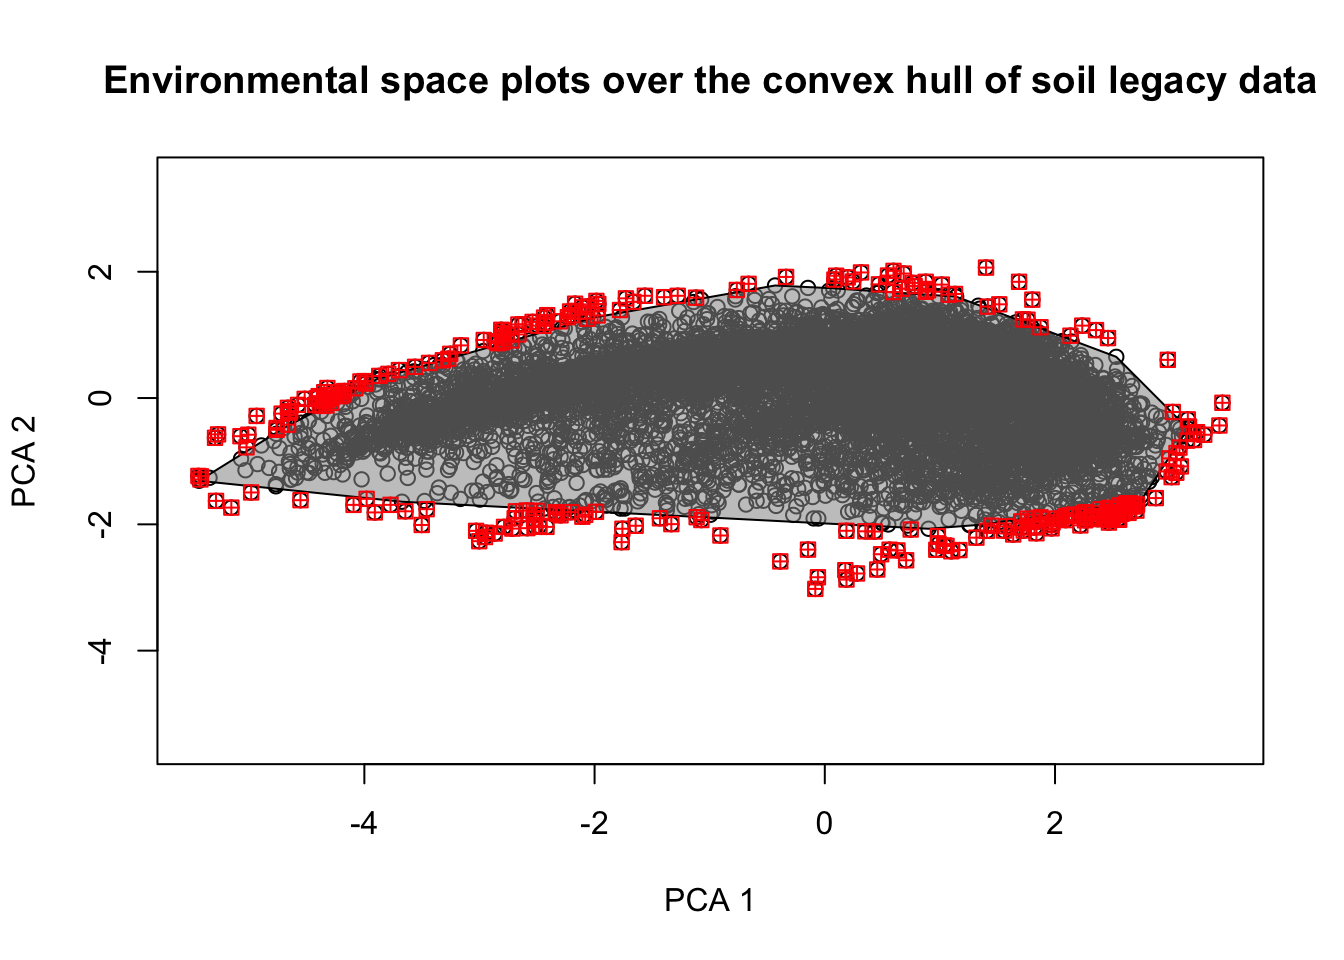
\includegraphics{Technical_Manual-on-Sampling-Design_files/figure-latex/compute_n_optimal_03-1.pdf}

Next Figure shows the distribution of covariates in the sample space.

\begin{Shaded}
\begin{Highlighting}[]
  \CommentTok{\# Merge data from number of samples, KL Divercence and \% representativeness }
\NormalTok{  results }\OtherTok{\textless{}{-}} \FunctionTok{data.frame}\NormalTok{(number\_of\_samples,klo\_samples,prop\_explained)}
  \FunctionTok{names}\NormalTok{(results)}\OtherTok{\textless{}{-}}\FunctionTok{c}\NormalTok{(}\StringTok{"N"}\NormalTok{,}\StringTok{"KL"}\NormalTok{,}\StringTok{"Perc"}\NormalTok{)}
  
  \CommentTok{\# Determine the minimum sample size to accounf for 95\% of representativeness of the covariate diversity}
\NormalTok{  optimal\_n }\OtherTok{\textless{}{-}}\NormalTok{ results }\SpecialCharTok{\%\textgreater{}\%}
    \FunctionTok{filter}\NormalTok{(Perc }\SpecialCharTok{\textgreater{}=}\DecValTok{95}\NormalTok{) }\SpecialCharTok{\%\textgreater{}\%} 
    \FunctionTok{filter}\NormalTok{(KL }\SpecialCharTok{==}\FunctionTok{min}\NormalTok{(KL) }\SpecialCharTok{|}\NormalTok{ N }\SpecialCharTok{==} \FunctionTok{min}\NormalTok{(N) }\SpecialCharTok{|}\NormalTok{ Perc }\SpecialCharTok{==}\FunctionTok{min}\NormalTok{(Perc) ) }\SpecialCharTok{\%\textgreater{}\%} 
    \FunctionTok{filter}\NormalTok{(N }\SpecialCharTok{==} \FunctionTok{min}\NormalTok{(N))}
\NormalTok{  optimal\_n}
\end{Highlighting}
\end{Shaded}

\begin{verbatim}
##     N         KL     Perc
## 1 150 0.06908217 95.88391
\end{verbatim}

\begin{Shaded}
\begin{Highlighting}[]
  \FunctionTok{plot}\NormalTok{(cov.dat[[}\DecValTok{1}\NormalTok{]])}
  \FunctionTok{points}\NormalTok{(p.dat\_I\_sp )}
\end{Highlighting}
\end{Shaded}

\begin{figure}
\centering
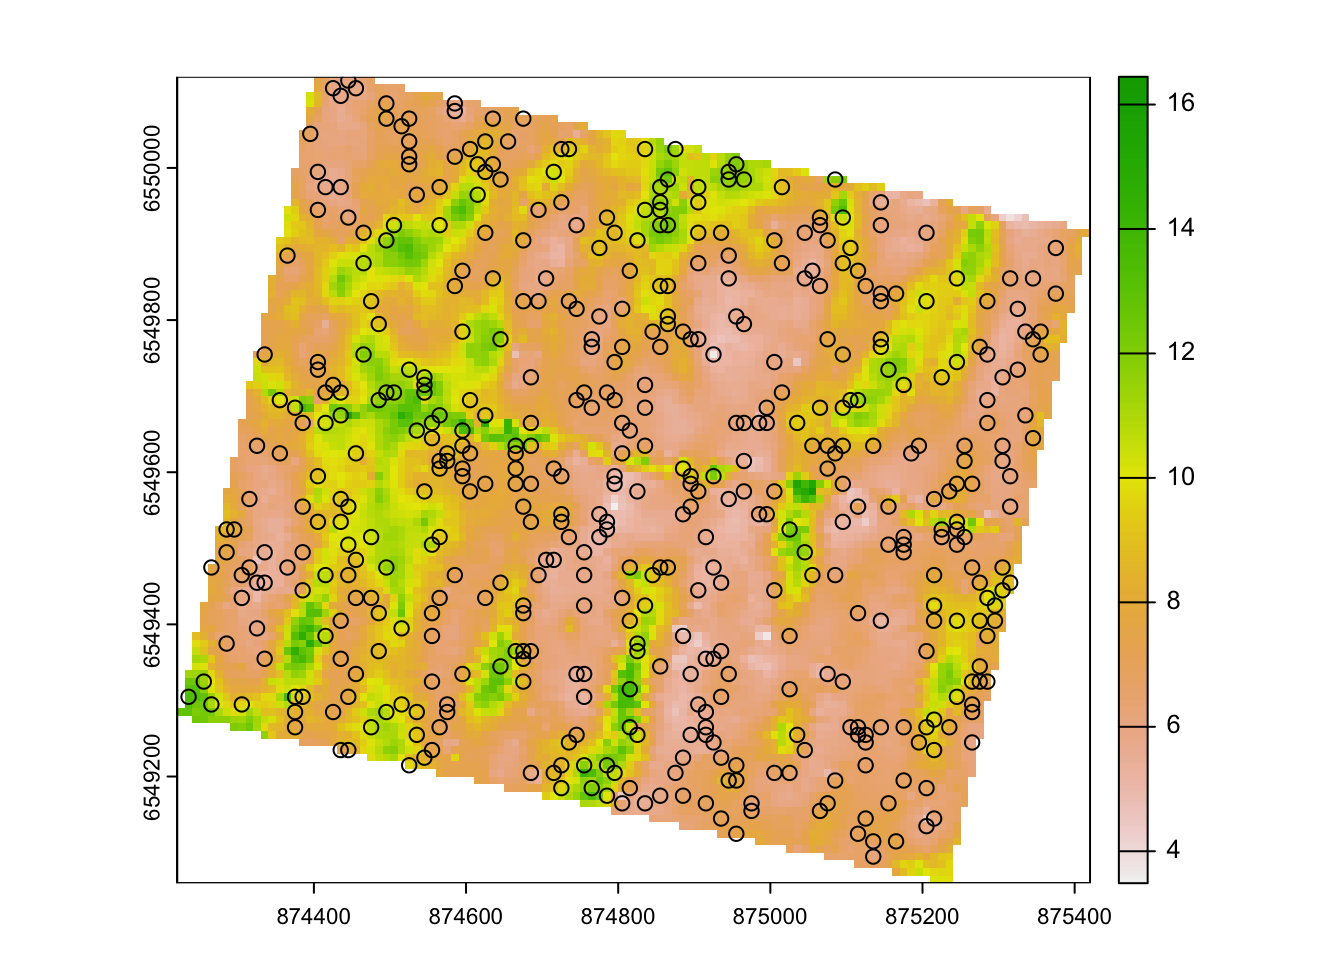
\includegraphics{Technical_Manual-on-Sampling-Design_files/figure-latex/plot_covandsamples_03-1.pdf}
\caption{(\#fig:plot\_covandsamples\_03)Covariates and distribution of samples}
\end{figure}

\begin{Shaded}
\begin{Highlighting}[]
\FunctionTok{plot\_ly}\NormalTok{(results,}
        \AttributeTok{x =} \SpecialCharTok{\textasciitilde{}}\NormalTok{N,}
        \AttributeTok{y =} \SpecialCharTok{\textasciitilde{}}\NormalTok{KL,}
        \AttributeTok{mode =} \StringTok{"lines+markers"}\NormalTok{,}
        \AttributeTok{type =} \StringTok{"scatter"}\NormalTok{,}
        \AttributeTok{name =} \StringTok{"KL divergence"}\NormalTok{) }\SpecialCharTok{\%\textgreater{}\%}
  \FunctionTok{add\_trace}\NormalTok{(}\AttributeTok{x =} \SpecialCharTok{\textasciitilde{}}\NormalTok{N,}
            \AttributeTok{y =} \SpecialCharTok{\textasciitilde{}}\NormalTok{Perc,}
            \AttributeTok{mode =} \StringTok{"lines+markers"}\NormalTok{,}
            \AttributeTok{type =} \StringTok{"scatter"}\NormalTok{,}
            \AttributeTok{yaxis =} \StringTok{"y2"}\NormalTok{,}
            \AttributeTok{name =} \StringTok{"\% Representativeness"}\NormalTok{)  }\SpecialCharTok{\%\textgreater{}\%}
  \FunctionTok{add\_trace}\NormalTok{(}\AttributeTok{x =} \SpecialCharTok{\textasciitilde{}}\NormalTok{optimal\_n}\SpecialCharTok{$}\NormalTok{N,}
            \AttributeTok{y =} \SpecialCharTok{\textasciitilde{}}\NormalTok{optimal\_n}\SpecialCharTok{$}\NormalTok{Perc,}
            \AttributeTok{yaxis =} \StringTok{"y2"}\NormalTok{,}
            \AttributeTok{mode =} \StringTok{"markers"}\NormalTok{,}
            \AttributeTok{name =} \StringTok{"Optimal N"}\NormalTok{,}
            \AttributeTok{marker =} \FunctionTok{list}\NormalTok{(}\AttributeTok{size =} \DecValTok{8}\NormalTok{, }\AttributeTok{color =} \StringTok{\textquotesingle{}\#d62728\textquotesingle{}}\NormalTok{,}\AttributeTok{line =} \FunctionTok{list}\NormalTok{(}\AttributeTok{color =} \StringTok{\textquotesingle{}black\textquotesingle{}}\NormalTok{, }\AttributeTok{width =} \DecValTok{1}\NormalTok{))) }\SpecialCharTok{\%\textgreater{}\%}
  \FunctionTok{layout}\NormalTok{(}\AttributeTok{xaxis =} \FunctionTok{list}\NormalTok{(}\AttributeTok{title =} \StringTok{"N"}\NormalTok{, }
                      \AttributeTok{showgrid =}\NormalTok{ T, }
                      \AttributeTok{dtick =} \DecValTok{50}\NormalTok{, }
                      \AttributeTok{tickfont =} \FunctionTok{list}\NormalTok{(}\AttributeTok{size =} \DecValTok{11}\NormalTok{)),}
         \AttributeTok{yaxis =} \FunctionTok{list}\NormalTok{(}\AttributeTok{title =} \StringTok{"KL divergence"}\NormalTok{, }\AttributeTok{showgrid =}\NormalTok{ F ),}
         \AttributeTok{yaxis2 =} \FunctionTok{list}\NormalTok{(}\AttributeTok{title =} \StringTok{"Representativeness (\%)"}\NormalTok{,}
                       \AttributeTok{overlaying =} \StringTok{"y"}\NormalTok{, }\AttributeTok{side =} \StringTok{"right"}\NormalTok{),}
         \AttributeTok{legend =} \FunctionTok{list}\NormalTok{(}\AttributeTok{orientation =} \StringTok{"h"}\NormalTok{, }\AttributeTok{y =} \FloatTok{1.2}\NormalTok{, }\AttributeTok{x =} \FloatTok{0.1}\NormalTok{,}
                       \AttributeTok{traceorder =} \StringTok{"normal"}\NormalTok{),}
         \AttributeTok{margin =} \FunctionTok{list}\NormalTok{(}\AttributeTok{t =} \DecValTok{50}\NormalTok{, }\AttributeTok{b =} \DecValTok{50}\NormalTok{, }\AttributeTok{r =} \DecValTok{100}\NormalTok{, }\AttributeTok{l =} \DecValTok{80}\NormalTok{),}
         \AttributeTok{hovermode =} \StringTok{\textquotesingle{}x\textquotesingle{}}\NormalTok{)  }\SpecialCharTok{\%\textgreater{}\%} 
  \FunctionTok{config}\NormalTok{(}\AttributeTok{displayModeBar =} \ConstantTok{FALSE}\NormalTok{) }
\end{Highlighting}
\end{Shaded}

\begin{figure}
\centering
\includegraphics{Technical_Manual-on-Sampling-Design_files/figure-latex/plot_KLfunction_03-1.pdf}
\caption{(\#fig:plot\_KLfunction\_03)KL Divergence and Proportion of Representativeness as function of sample size}
\end{figure}

\hypertarget{references}{%
\chapter*{References}\label{references}}
\addcontentsline{toc}{chapter}{References}

  \bibliography{references.bib}

\end{document}
